\documentclass{article}

\usepackage{blindtext}
\usepackage{amsmath}
\usepackage{graphicx}
\usepackage{subcaption}
\usepackage{float}
\usepackage[ruled,vlined]{algorithm2e}
\usepackage{hyperref}

\bibliographystyle{unsrt}

\usepackage{booktabs}
\usepackage{array}



\begin{document}

\title{Online navigation with neuromodulation-based Hebbian plasticity}
\author{Krubeal Danieli}

\maketitle

\newpage

\tableofcontents

\newpage


\section{Introduction}
% \hfill \break
% \vspace {0.5cm}

% brief introduction to decision making and the brain.
The ability to make decisions for long-term reward maximization is a fundamental aspect of cognition. The brain has evolved specialized and interconnected regions to implement this behaviour under the constraints of biology.

% bridge between decision making and the k-armed bandit problem.
Well-studied ecological settings of decision-making are foraging tasks, such as food search. In this problems, the agent is usually asked to choose between different options to maximize an expected reward.
In nature, animals have been shown to exhibit different strategies depending on context.
\textit{Matching behaviour} is a well-known phenomenon in which the animal's decision patterns are proportional to the reward probability of the available options.
Such behaviour is thought to result from the trade-off between exploration and exploitation \cite{suttonReinforcementLearningProblem1998, nivEvolutionReinforcementLearning2002}.
In fact, this is a well known phenomenon in the reinforcement learning literature, in which an agent is faced with the dilemma of exploring new alternatives, potentially more rewarding, or exploiting known options, despite being possibly sup-optimal.

A popular formalization of these type of tasks is the \textit{multi-armed bandit} problem (MAB) \cite{averbeckTheoryChoiceBandit2015}. This setting is usually described in terms of a slot machine endowed with $K$ distinct arms, also called levers.
During a round, the agent selects one of the arms and collects a reward $R$ according to an unknown reward probability specific to the chosen arm.
The goal is simply to maximize the total reward after a given number of steps, which is achieved by effectively updating a selection policy after each round.
This problem has been extensively studied in the context of reinforcement learning, and it is considered a fundamental building block for more complex tasks \cite{suttonReinforcementLearningProblem1998}.

% brief introduction of the k-armed bandit problem and previous algorithms.
% \subsection{Related work}
% \hfill \break
There exist various flavours of this problem, with the simplest having a stationary reward distribution.
Over the years, several algorithms have been proposed, alongside with their theoretical guarantees.
In this regard, Thompson sampling is a popular algorithm that has been shown to achieve near-optimal regret bounds in the stochastic setting \cite{agrawalAnalysisThompsonSampling2012, kaufmannThompsonSamplingAsymptotically2012}.
This approach relies on Bayesian optimization, where the goal is to maintain a posterior distribution over the reward probabilities of the actions, and select actions accordingly.
Another popular algorithm is Upper Confidence Bound (UCB), which has been shown to achieve near-optimal regret bounds in the adversarial setting \cite{auerFinitetimeAnalysisMultiarmed2002}.
The approach is based on the idea of maintaining an upper limit on the reward probabilities of the actions, and select actions accordingly.
Other successful algorithms are $\epsilon$-Greedy and VDBE \cite{gittinsBanditProcessesDynamic1979, banMultifacetContextualBandits2021, tokicAdaptiveEGreedyExploration2010, tokicValueDifferenceBasedExploration2011}.

% why bio-plausibility is important
Nonetheless, put aside their marked success, they bear little resemblance to actual neuronal dynamics, besides lacking a clear functional similarity to brain regions.
Indeed, the interest in bio-inspired algorithms has seen a rise in recent years. One of the reasons is the optimization of energy usage, through the design of models with a better tradeoff between performance and power consumption \cite{EvaluationBioInspiredModels}, and possibly running on specialized neuromorphic hardware \cite{ReviewNeuroscienceInspiredMachine}.
Other important advantages include novel algorithmic approaches employed by biological brains such as neural networks and predictive coding, which have been shown to be reach state of the art in several tasks and deal with the so-called \textit{machine-challenging tasks} (MCTs) \cite{schmidgallBraininspiredLearningArtificial2024, hassabisNeuroscienceInspiredArtificialIntelligence2017, leeBraininspiredPredictiveCoding2022}.
Lastly, bio-inspired models can be used to improve algorithmic intepretability, namely understanding what is actually happening behind the scene, and make more direct comparison with real biological dynamics and components \cite{liuSeeingBelievingBrainInspired2023}.

\hfill \break
% aim of the work
\indent In this work, we aimed at improving the biological plausibility of algorithms in the context of the multi-armed bandit problem by proposing a new model based on rate neurons and synaptic plasticity.
Additionally, we optimized the hyper-parameters of the model through an evolution search, showing the convergence to solutions in line with experimental observations.
The benchmarks we chose are stochastic bandit problems, more challenging variants of the original task endowed with \textit{concept drift}, where the reward distribution changes over time \cite{garivierUpperConfidenceBoundPolicies2008, besbesStochasticMultiArmedBanditProblem2014, cavenaghiNonStationaryMultiArmed2021}.

% brief overview of the model
The architecture of our model consists of two connected neuronal layers, both with as many neurons as the arms of the bandit task.
The first layer is inspired by the functionality of the orbitofrontal cortex (OFC), and its scope is to maintain an active representation of the arms weighted by the input from the second layer. These two areas are thought to be involved in motivation and representation of the expected value of the actions, either positive or negative \cite{odohertyAbstractRewardPunishment2001, ricebergRewardStabilityDetermines2012, tremblayRelativeRewardPreference1999}, action selection in uncertain environments \cite{elliottDissociableFunctionsMedial2000}, and contextual processing \cite{frankAnatomyDecisionStriatoorbitofrontal2006}.
The second layer is instead modeled after the ACC, and it is meant to represent the value of the arms. Its input connections are updated through a learning rule dependant on the reward history and current connectivity pattern.

% main motivations
Our model features two important aspects of the brain during decision making. Firstly, the option selection process itself is implemented as a dynamical interaction between neural populations, similarly to bump attractor networks for perceptual cognition \cite{carrollEncodingCertaintyBump2014, esnaola-acebesBumpAttractorDynamics2021}.
The final choice of the arm is achieved by the agreement or disagreement between the two populations, and it depends on their underlying value representation \cite{bariDynamicDecisionMaking2021, houstonMatchingBehavioursRewards2021}.

Secondly, plasticity is based on a non-associative learning rule, endowed with a non-linear kernel for the weight update term.
Behind this design choice there is our hypothesis that the scale of the synaptic update should vary non-linearly according to its magnitude.
This consideration is aligned with the idea that the learning rate is a parameter specific to each neuron. This synapse-type specific plasticity (STSP) \cite{larsenSynapsetypespecificPlasticityLocal2015} is a function of the resources available at the synaptic button and its state, including the size \cite{blackmanTargetcellspecificShorttermPlasticity2013, bartolHippocampalSpineHead2015, arielIntrinsicVariabilityPv2012}.
This approach has been already adopted in several computational architectures, for instance in spiking neural networks \cite{inglisModulationDopamineAdaptive2021} and for synaptic metaplasticity \cite{iigayaAdaptiveLearningDecisionmaking2016}.
Lastly, there is experimental evidence that this adaptation function might be covered by dopamine \cite{toblerAdaptiveCodingReward2005}.
Indeed, its involvement in calculating prediction errors and reward signaling is well established \cite{schultzNeuralSubstratePrediction1997}, as well with its modulation of  high-level cortical networks like the PFC \cite{didomenicoDopaminergicModulationPrefrontal2023, lohaniDopamineModulationPrefrontal2019, dardenneRolePrefrontalCortex2012}.




% \newpage



\section{Methods}

% brief introduction of the k-armed bandit problem and previous algorithms.
\subsection{Related work}
% overview of the main solutions proposed in the literature from a computational perspective.
There exists various flavours of this problem, with the simplest having a stationary reward distribution, while the more challening ones have have \textit{concept drift}, where the reward distribution changes over time.
Over the years, several algorithms have been proposed, alongside with their theoretical guarantees. In this regard, Thompson sampling is a popular algorithm that has been shown to achieve near-optimal regret bounds in the stochastic setting \cite{agrawalAnalysisThompsonSampling2012}, which 
a Bayesian approach  the idea of maintaining a posterior distribution over the reward probabilities of the actions, and selecting actions according to the posterior distribution. Another popular algorithm is the Upper Confidence Bound (UCB) algorithm, which has been shown to achieve near-optimal
regret bounds in the adversarial setting \cite{auerFinitetimeAnalysisMultiarmed2002}. The algorithm is based on the idea of maintaining an upper confidence bound on the reward probabilities of the actions, and selecting actions according to the upper confidence bound.
\\
% outline of lack of bio-realism and what we currently know about how the brain might solve this task.
Despite the success of these algorithms in solving the k-armed bandit problem, they lack biological plausibility. In contrast, the brain has evolved a complex network of interconnected regions that work together to solve this task. In particular, the dopamine-acetylcholine system has been shown to
play a crucial role in learning and decision making \cite{dayanDecisionTheoryReinforcement2008}.

% mathematical formulation of the k-armed bandit problem.
\subsection{Binomial K-armed bandit problem}
\hfill \break
\noindent The standard formulation of the task is structured as a set of $\{1\dots K\}$ levers (or arms), with an associated reward distribution $\mathbf{p}=\{p_{1}, \ldots p_{K}\}$. At each iteration, the agent pulls a lever and collect a possible reward drawn as a Bernoulli variable $R\sim
\mathcal{B}(\{0,1\},p_{k})$. The agent's objective is maximizing the total reward
$\sum^{T}_{t} R_{t}$, after a certain number $T$ of trials. Importantly, the agent is unaware of the true reward probability distribution, and thus has to make its decisions following a certain policy, usually denoted as $\pi$. In the reinforcement learning literature, the policy is often defined as
a distribution over the actions, here the levers $K$, given the current state, which in this case can be the history of past actions and rewards up to time $t\leq T$. Given the inherent stochasticity of the feedbacks from the environment, the definition of the policy is affected by the so-called
exploration-exploitation trade-off, which here is phrased as the contrast between the option of the lever with the known highest expected reward versus the option to explore other levers, so to gather more information. A common approach is the $\epsilon-$greedy policy, where the choice to explore is
selected with a probability $\epsilon$. Moreover, it is often preferable to have a more explorative behaviour early during the training, with the intent to have a good sample size for the empirical reward distribution, which can be later exploited for maximizing reward.\\
Another important concept in multi-armed bandit problems is the \textit{regret}. Intuitively, it is defined as the deviation of the total reward obtained by the agent from the optimal reward that could have been obtained by always choosing the lever with the highest expected reward. Formally, the regret is defined as:
\begin{equation}
    \rho=R^{*} - \sum^{T}_{t} R_{t}
\end{equation}

\noindent where $R^{*}$ is the reward obtained by always choosing the lever with the highest expected reward $R^{*}=T\max_{k}\{p_{k}\}$, and $R_{t}$ is the empirical reward obtained up to time $t$ by following policy $\pi$ as $R_{t}=\sum^{T}_{t=1}\pi_{\theta}(t)$.
The regret is a measure of the performance of the agent, and it is often used to compare different algorithms. The goal of the agent is to minimize the regret, and thus maximize the total reward.

\hfill \break
\textbf{Goal} \\
\noindent The setting we consider in this work is a non-stationary environment with Binomial rewards. In particular, the agent is evaluated over a number $T_{\text{trials}}$ of \textit{trials}, each composed by an arbitrary number $T$ of \textit{rounds}; each \textit{trial} is characterized by a different
reward distribution $\mathbf{p}\sim\mathcal{U}(0,1)^{K}$ (although in practice the bounds have been set to $(0.1, 0.8)$ such that the distributions are less trivial). \\
\noindent Our goal in this work is to investigate the performance of the agent in a non-stationary environment with Binomial reward distributions, meaning that its underlying distribution changes over time. We choose this setting as it resembles an ecological scenario in which an animal has to forage in a patchy environment, where the reward of a given patch can change over time.
We will consider two types of non-stationarity: \textit{zero} and $\epsilon$-steps. In the first case, the reward distribution changes at a given time step. In the second case instead, the reward distribution changes gradually over time; in practice, it tends to a target distribution
$\pi_{\text{trg}}$ which is changed once the distance is below a threshold as $\vert \pi_{\text{trg}} - \pi_{t}\vert < \epsilon$.
We will investigate the performance of the model in both settings, and compare it to the common benchmark algorithms.

% review of previous work

%% description of the model architecture.
%\subsection{Model architecture}
%\hfill \break
%Our model is inspired by the architecture of the dorsolateral pre-frontal (DLPFC) cortex and orbitofrontal-basal ganglia system (OFC-BG), and it is designed to solve the k-armed bandit problem through the dynamics occuring in the memory neural space.
%The model is composed of two main components: a memory structure, the DLPFC (hereforth referenced as $M$), and an executive structure, the prefrontal cortex-basal ganglia (referenced as $C$). A decision is made when the active trace of an option in $M$ is sufficiently stable, condition that requires the $C$ to have selected the same option.
%$M$ is implemented as a recurrent neural network with the ability to form memory traces, while $C$ implements executive functions such as top-down attention.

%%figure
%\begin{figure}[ht]
%    \centering
%    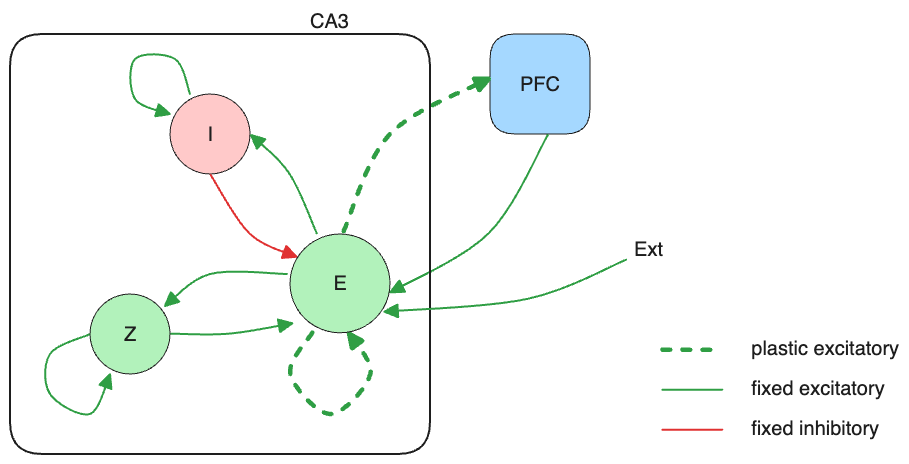
\includegraphics[width=0.6\textwidth]{figures/model_architecture_2.png}
%    \caption{\textsc{Model architecture - }\textit{$M$ is composed of three populations: excitatory (E), inhibitory (I) and auxiliary (Z), memory consolidation occurs only in the recurrent connection of population E. The $C$ is a mixed model, with a network and symbolic part, its afferent
%    connection from $M$ are plastic.}}
%    \label{fig:model_architecture1}
%\end{figure}


%% ------ HPC ------ %
%\hfill \break
%\noindent \textbf{Working Memory ($M$)}\\
%\noindent $M$ receives inputs from $C$ and from an external source, as illustrated in figure \ref{fig:model_architecture1} above. The external current is an aspecific spike input with a fixed rate of $300$Hz targeting all $M$'s neurons.
%The intent of this global excitation is to be strong enough to increase the activity in the recurrent network but also weak enough to allow drifts in the activity space influenced by the memory attractors. Then, $C$ stimulations further modulate the dynamics by providing a selective input to specific subnetworks. \\
%Another feature of $M$ is a working memory mechanism, which has the role of keeping active the neural pattern corresponding to the selected action (lever) and suppressing the others while waiting for the external feedback to arrive. This mechanism is implemented by a adding to the main
%excitatory population $E$ an inhibitory
%population $I$ and an auxiliary excitatory $Z$. The rationale behind this architecture is to have a way to bound the activity in $E$ through a proportional inihibition from $I$. However, when an attractor gets strong enough to meaningfully engage the population $Z$, which adds extra stimulation to
%the neurons involved in the memory, the inhibition $I$ silences effectively only the neurons not part of the active trace. \\
%% equations %
%The dynamics of $M$ are defined in terms of an internal variables $x^{\text{E}}_{t}$, which is the activity of the excitatory population $E$. In particular, the spiking behavour is described by a Spike Response Model (SRM) neuron model, which is based on a a series of kernels of the EPSP (and
%IPSP) for the relevant neuronal processes:
%\begin{equation}
%    \tau x^{E}_{i}=E_{\text{rest}}-x^{E}_{i}+\chi(t-t^{f}_{i}) + h^{EE}_{i} + h^{IE}_{i} + h^{ZE}_{i} + I^{\text{P}}_{i} + I^{\text{ext}}_{i}
%\end{equation}
%\noindent where $\chi$ is the kernel for the refractory period, $I^{\text{P}}_{i}$ is the projection from $C$, $I^{\text{ext}}_{i}$ is the external input, and $h^{EE}$ is the kernel for the recurrent connections, which define the contributions of spike trains $S^{E}_{j}$ from neighboring neurons:
%\begin{equation}
%    h^{EE}_{i}(t)=\sum\limits_{j}^{N^{E}}w_{ij}\int^{\infty}_{0}\kappa(s)S^{E}_{j}(t-s)ds
%\end{equation}
%\noindent where $\kappa$ is the synaptic kernel, and $w_{ij}$ is the synaptic weight for the recurrent connections $W^{EE}$. The kernels $h^{IE}$ and $h^{ZE}$ are defined similarly, but for the inhibitory and auxiliary populations, respectively. \\ The resulting spike train is then obtained by
%sampling from a Poisson process whose intensity is the non-linearly bounded internal variable:
%\begin{equation}
%    S_{i,t}\sim \mathcal{B}(\sigma_{\alpha, \beta}(x^{E}_{i}))
%\end{equation}
%\noindent where $\mathcal{B}$ is a Bernoulli sample, and $\sigma$ is a generalized sigmoid parametrized by $\alpha, \beta$. Each spike then updates, for each neuron $i$, its last spike-time $t^{f}_{i}$, used to calculate the EPSP in the SRM model.


%% ----- PFC ------ %

%\hfill \break
%\noindent \textbf{Executive Control ($C$)}\\
%\noindent $C$ receives afferent projections from $M$, which deliver the information about the currently active traces. Initially, these connections are set to zero, and $C$ is not influenced by $M$ activity, meaning it will settle for random decisions. Next, as the feedbacks start to accumulate,
%the afferent connections, which are plastic, get consolidated, encoding for a proxy of the value of the current option. \\
%$C$ defines its activity by means of a small neural network layer of leaky spiking neurons, which integrate the activity coming from $M$ and the an evaluation of the current options' value which can be considered a \textit{value function}, implemented through a non-linear function $\phi^{\text{P}}$:
%\begin{equation}
%    \tau \dot{u}^{\text{P}}_{i} = -u^{\text{P}}_{i} + \phi^{\text{P}}\left(W^{\text{HP}}_{i}\right)h^{\text{EP}}
%\end{equation}\label{pfc_x}
%From which the output is defined as follows:
%\begin{equation}
%    a_{i} = \text{relu}\left[\sigma_{\beta}\left(u_{i}\right) \mathcal{H}\left(h^{\text{EP}} - \theta_{1}\right)\right]
%\end{equation}
%\noindent where $\sigma_{\beta}$ is a generalized softmax parametrized by $\beta$, and $\mathcal{H}$ is the Heaviside function with threshold $\theta_{1}$.


%% ----- option selection ------ %

%% description of the model dynamics
%%\hfill  \break
%\subsubsection{Option selection}
%\noindent The decision making process is such that an output is well-defined only when $M$ is in a stable memory attractor that underlies an option that has also been selected by $C$. \\
%The excitatory population $E$ has around $\sim 50$ neurons for encoding each option, which has an average EPSP current $h^{\text{H}}_{k}$ ().where $\varphi_{K}$ is a function that compress the activity of the $N^{E}$ excitatory CA3 network into the vector of average activity for the traces $x^{\text{H}}_{t}$ of the $K$ memories.


%% ----- LEARNING ------ %

%\subsubsection{Learning rule}

%% - M - %
%In $M$, plasticity occurs only in the recurrent connections of the excitatory population $E$, with the scope of consolidating the memory traces. The synaptic weights are updated according to an Oja-style rule, that is dependent on the pre and post-synaptic activity, and on the current weight
%value. However, here it is introduced two modulation terms, $\text{DA}, \text{ACh}\in\{0,1\}$, which determines the direction of the update in either potentiation or depression respectively. The update in matrix form is given by:

%\begin{equation}
%    \Delta W^{\text{EE}} = \eta_{+}\text{DA}\,(W^{\text{EE}}_{\text{max}}-W^{\text{EE}})\,\Delta^{\text{hebb}} - \eta_{-}\text{ACh}\,W^{\text{EE}}\,\Delta^{\text{hebb}}
%\end{equation}

%\noindent where $\eta_{+}, \eta_{-}$ are the learning rates, and $W^{\text{EE}}_{\text{max}}$ is the maximum weight value. The Hebbian term $\Delta^{\text{hebb}}$ is calculated through a Gaussian filter with width $\tau_{\text{ps}}$ and shape $\phi(t)=e^{-0.5\,(\frac{t}{\tau_{\text{ps}}})^2}$ over the time of the last spike of the pre and post-synaptic neurons $i,j$:
%\begin{equation}
%    \Delta^{\text{hebb}}_{ij} = \phi(t-\mathbf{t}^{f}_{i})\,\phi(t-\mathbf{t}^{f}_{j})^{T}
%\end{equation}

%\noindent Then, for homeostatic reasons, the weights are clipped in $\left(0, W^{\text{EE}}_{\text{max}}\right)$ and normalized such that the total input remains constant $w_i=\bar{w}^{EE}\,\frac{w_i}{\sum\limits_{j}w_{ij}}$.

%\hfill \break
%% - PFC - %
%As for the $C$, learning happens in the afferent projections from $M$, with the intent of encoding the value of the currently active option. As before, the update is dependent on the valence of the feedback, gated by the dopamine and acetylcholine signals. However, unlike $M$, the specific rule
%is defined only in terms of the pre-synaptic activity and the current weight value, and it takes the form of a mixture of Gaussians $\Theta_{\pm}$, with different parameters for potentiation and depression respectively. The update is given by:
%\begin{equation}
%    \Delta W^{\text{HP}} = \eta\,\phi(t-\mathbf{t}^{f})\,\left[\text{DA}\,\Theta_{+}(W^{\text{HP}}) - \text{ACh}\,\Theta_{-}(W^{\text{HP}})\right]
%\end{equation}

%\noindent where $\textbf{t}^{f}$ is the time of the last spike of the pre-synaptic neuron, and $\eta$ is the learning rate.


%% ----- OPTIMIZATION ------ %

%\subsubsection{Performance}

%\noindent Given the model architecture, the performance of the agent is significantly determined by the $C$ dynamics, which biases the $M$ activity to pivot towards a preferred option. In particular, the shape of the $C$'s synaptic plasticity function $\Theta_{\pm}$ enables a non-linear
%consolidation of the afferent connections and a specific rate of change for potentiation and depression, with the scope of differentiating between small, medium, and large weights. Similarly, the non-linearity of the \textit{value function} $\phi^{\text{P}}$ is crucial in determining the influence
%on the $M$ activity while considering the current evaluation of the options. \\
%Both the synaptic plasticity function and the value function are implemented as a mixiture of Gaussians:

%\begin{equation}
%\phi_{2}(x)=r\,\gamma_{1}\exp\left[-\left(\frac{x-\mu_1}{\sigma_{1}}\right)^{2}\right]+(1-r)\,\gamma_{2}\exp\left[-\left(\frac{x-\mu_2}{\sigma_{2}}\right)^{2}\right]
%\end{equation}
%with function-specific parameters: $\{r, \gamma_{1}, \gamma_{2}, \mu_{1}, \mu_{2}, \sigma_{1},\sigma_{2}\}$.

%\hfill \break
%The optimization of the parameters has been carried out through an evolutionary search using the Covariance Matrix Adaptation Evolution Strategy (CMA-ES) algorithm, which is a stochastic optimization method particularly suited for high-dimensional and non-linear optimization problems. 




\newpage
% 
\subsection{Model description}
The model is constructed as a rate network of two populations of neurons \textit{M} and \textit{P}, the former representing the memory trace of the \textit{K} available options (\textit{i.e.} the bandits), and the latter representing the value of the options under the current policy.
More formally, the model is described by a set of coupled ordinary differential equations (ODEs) that capture the decision-making process in two distinct neural spaces.
The first equation tracks the evolution of the neural activity $\textbf{u}$ of \textit{M}, while the second tracks the activity $\textbf{v}$ of the \textit{P}. The time constants $\tau$ are the same for both equations and are set to $\tau = 10$ ms.


\begin{equation}
\begin{aligned}
    \tau \dot{\textbf{u}}&= -\textbf{u} + \textbf{v} + \textbf{I}_{\text{ext}} \\
    \tau \dot{\textbf{v}}&= -\textbf{v} + \textbf{z} \odot\textbf{u}
\end{aligned}
\end{equation}

\noindent The external input $\textbf{I}_{\text{ext}}$ is a constant input that is used to set the initial conditions of the neural activity $\textbf{u}$.
The term $\textbf{z}$ is a vector that weights the contribution of the active options $\textbf{u}$ to the value representation $\textbf{v}$, and functionally it is the core of the policy adopted by the model.
In practice, $\textbf{z}$ defined as a function of the synaptic weights $\textbf{W}^{MP}$ from \textit{M} to \textit{P} as $\textbf{z} = \Phi_v(\textbf{W}^{MP})$. Importantly, the connections are not fully connected, but rather are simply one-to-one mapping between the corresponding neurons in each
population, such that the weight matrix $\textbf{W}^{MP}$ is simply a matrix $K\times 1$, namely a vector.
The function $\Phi_v$ is a chosen to be a sum of a generalized sigmoid and a Gaussian, whose contributions are weighted by a parameter $r$:

\begin{equation*}
    \Phi_v(x) = r\gamma_{1} \frac{1}{1 + e^{-\beta(x-\alpha)}} + (1-r)\gamma_{2} \exp\left(-\frac{(x-\mu)^2}{2\sigma^2}\right)
\end{equation*}

\noindent The motivation behind this choice is to express a function that possesses a bounded region (depending on $\mu,\,\sigma$) at a high/low peak (depeding on the value of $\gamma_{2}$), and a continuous transition to a constant value (depending on the steepness of the sigmoid $\beta$, shift
$\alpha$, and intensity $\gamma_{1}$).

\hfill \break
\textbf{Option selection} \\
The decision-making process within a single round is structured in two distinct phases. Initially, the model receives a constant external input targeting all neurons in the memory population \textit{M} equally.
During this phase, $I_{\text{ext}}$ works as an equilibrium value while the reciprocal interactions with population \textit{P} push $\textbf{u}$ to different values, depending on the current policy encoded in $\textbf{z}$. However, in the early rounds the weights $\textbf{W}^{MP}$ are zero, and thus
the contribution from \textit{P} is null. After a fixed amount of time $\sim 5 \text{s}$, the second phase begins. Here, the external input is removed and the model is left to evolve autonomously, and since there are no recurrent connections in neither population the dynamics is entirely driven by their coupling. \\
A selection $\hat{k}$ is sampled after another fixed amount of time $\sim 5 \text{s}$, and it is defined according to the following rule:

\begin{equation*}
    \hat{k} =
    \left\{
        \begin{array}{ll}
            \text{argmax}_{k}\{\textbf{v}\} & \text{\textit{if}}\; \text{argmax}_{k} \{\textbf{v}\} = \text{argmax}_{k} \{\textbf{u}\} \\
            \text{random}(K) & \text{\textit{otherwise}}
        \end{array}
    \right.
\end{equation*}

\noindent The selection rule is simple: if the value representation $\textbf{v}$ is in agreement with the memory trace $\textbf{u}$, then the option with the highest value is selected. Otherwise, a random option is chosen. This rule is a way to express the exploration-exploitation trade-off, and it is dependent on the current policy $\textbf{z}$.

\hfill \break
\textbf{Learning} \\
Given a selected option, the environment (bandit) samples and returns a reward $R\in [0, 1]$.
Then, the connections $\textbf{W}^{MP}$ for the neuron corresponding to the option $k$ are updated according to the following plasticity rule:

\begin{equation}
    \Delta \textbf{W}^{MP}_{k} = \tilde{\eta}_{k} \left(R\cdot W^{+}- \textbf{W}^{MP}_{k}\right)
\end{equation}

\noindent
Where $W^{+}$ is a constant value that sets the upper bound for the synaptic weights, and it is set to $W^{+} = 5$, while $\tilde{\eta}_{k}$ is the learning rate for the option $k$ determined by a function of the current weights $\textbf{W}^{MP}_{k}$ and its shape is the same as $\Phi_{v}$, but with
different parameters.


  % minimal model
%\newpage

\section{Experiments}

The model has been tested in a series of benchmark environments, each with a different number of arms and reward distributions. The performance has been compared with the following algorithms: Random Baseline, Upper-Confidence Bound (UCB), Thompson Sampling, and Epsilon-Greedy.

% Description of the environments
\subsection{Game variants} %\textbf{YEAH BUDDY WORK ON THIS A LIL MORE}

% \noindent The game environments considered in this work are non-stationary K-Armed Bandits with Binomial rewards.
% In particular, the agent is evaluated over a number $T_{\text{trials}}$ of \textit{trials}, each composed by an arbitrary number $T_{\text{rounds}}$ of \textit{rounds}; each \textit{trial} is characterized by a different reward distribution $\mathbf{p}\sim\mathcal{U}(0,1)^{K}$ (although in practice the bounds have been set to $(0.1, 0.9)$ such that the distributions are less trivial).
\noindent Our goal in this work is to investigate the performance of the agent in a non-stationary environment with Binomial reward distributions, meaning that its underlying distribution changes over time \footnote{Since the arm probabilities are not normalized to $1$, it is
technically improper to call them \textit{probability distributions}; we will therefore refer to either \textit{probability} or \textit{distribution} separately at any given time for avoiding confusion.}
We choose this setting as it resembles an ecological scenario in which an animal has to forage in an environment with food (reward) is distributed over a set of fixed locations, but whose occurrence probability can change over time.
More specifically, we used four different variants obtained by introducing different types of non-stationarity: piecewise constant, uniformly changing, sinusoidally changing, and sinusoidally changing plus piecewise constant.
The reason for this choices is to test the model performance under different speed and uniformity of the distribution changes.
Figure \ref{fig:envs} visually illustrates their specificities.

\hfill \break
\noindent \textbf{Piecewise stationary environment} [\textsc{KAB-P}]\\ Within a trial the reward distribution is stationary and it is drawn from a uniform $\mathbf{p}=\mathcal{U}(0, 1)^{K}$. At the end of each trial $i$ it is drawn a new distribution $\mathbf{\mathbf{p}}_{i} \to \mathbf{\mathbf{p}}_{i+1}$ \cite{qiForcedExplorationBandit2023}.

\hfill \break
\noindent \textbf{Piecewise stationary environment with drift} [\textsc{KAB-D}]\\ At the very beginning, the reward distribution $\mathbf{p}$ is sampled from a uniform $\mathbf{p}=\mathcal{U}(0, 1)^{K}$. Then, it changes gradually over the rounds, tracked as time $t$, such that its values tend towards a target distribution $\mathbf{q}_{i}$ as $\tau_{p}\dot{\mathbf{p}}_{t}=\mathbf{q}_{i}-\mathbf{p}_{t}$.
Here, $\dot{\mathbf{p}}$ is the time derivative of the distribution and $\tau_{p}$ is its time constant.
Once the distance is below a threshold $\delta$ as $\vert \mathbf{q}_{i} - \mathbf{p}_{t}\vert < \delta$, the target distribution is changed to a new one $\mathbf{q}_{i}\to\mathbf{q}_{i+1}$. In this variant, there are no proper trials but the target distribution keep changing until a maximum number
of rounds is reached.

\hfill \break
\noindent \textbf{Sinusoidal distribution shift} [\textsc{KAB-$\sin$}]\\ The reward distribution changes over rounds, with the probability of each arm following a sine wave with a specific frequency $f_{k}$, phase $\lambda_{k}$ and amplitude $1$. At any given time $t$, the distribution is $\mathbf{p}_{t}=\{\sin(2\pi f_{k} t+\lambda_{k})\text{  for }k=1\ldots K\}$.

\hfill \break
\noindent \textbf{Partial sinusoidal distribution shift} [\textsc{KAB-$\sin$P}]\\ Identical to the sinusoidal distribution shift, but only a subset of the arms changes sinusoidally while the rest is kept at a constant value and the distribution is not normalized.


\begin{figure}[h]
    \centering
    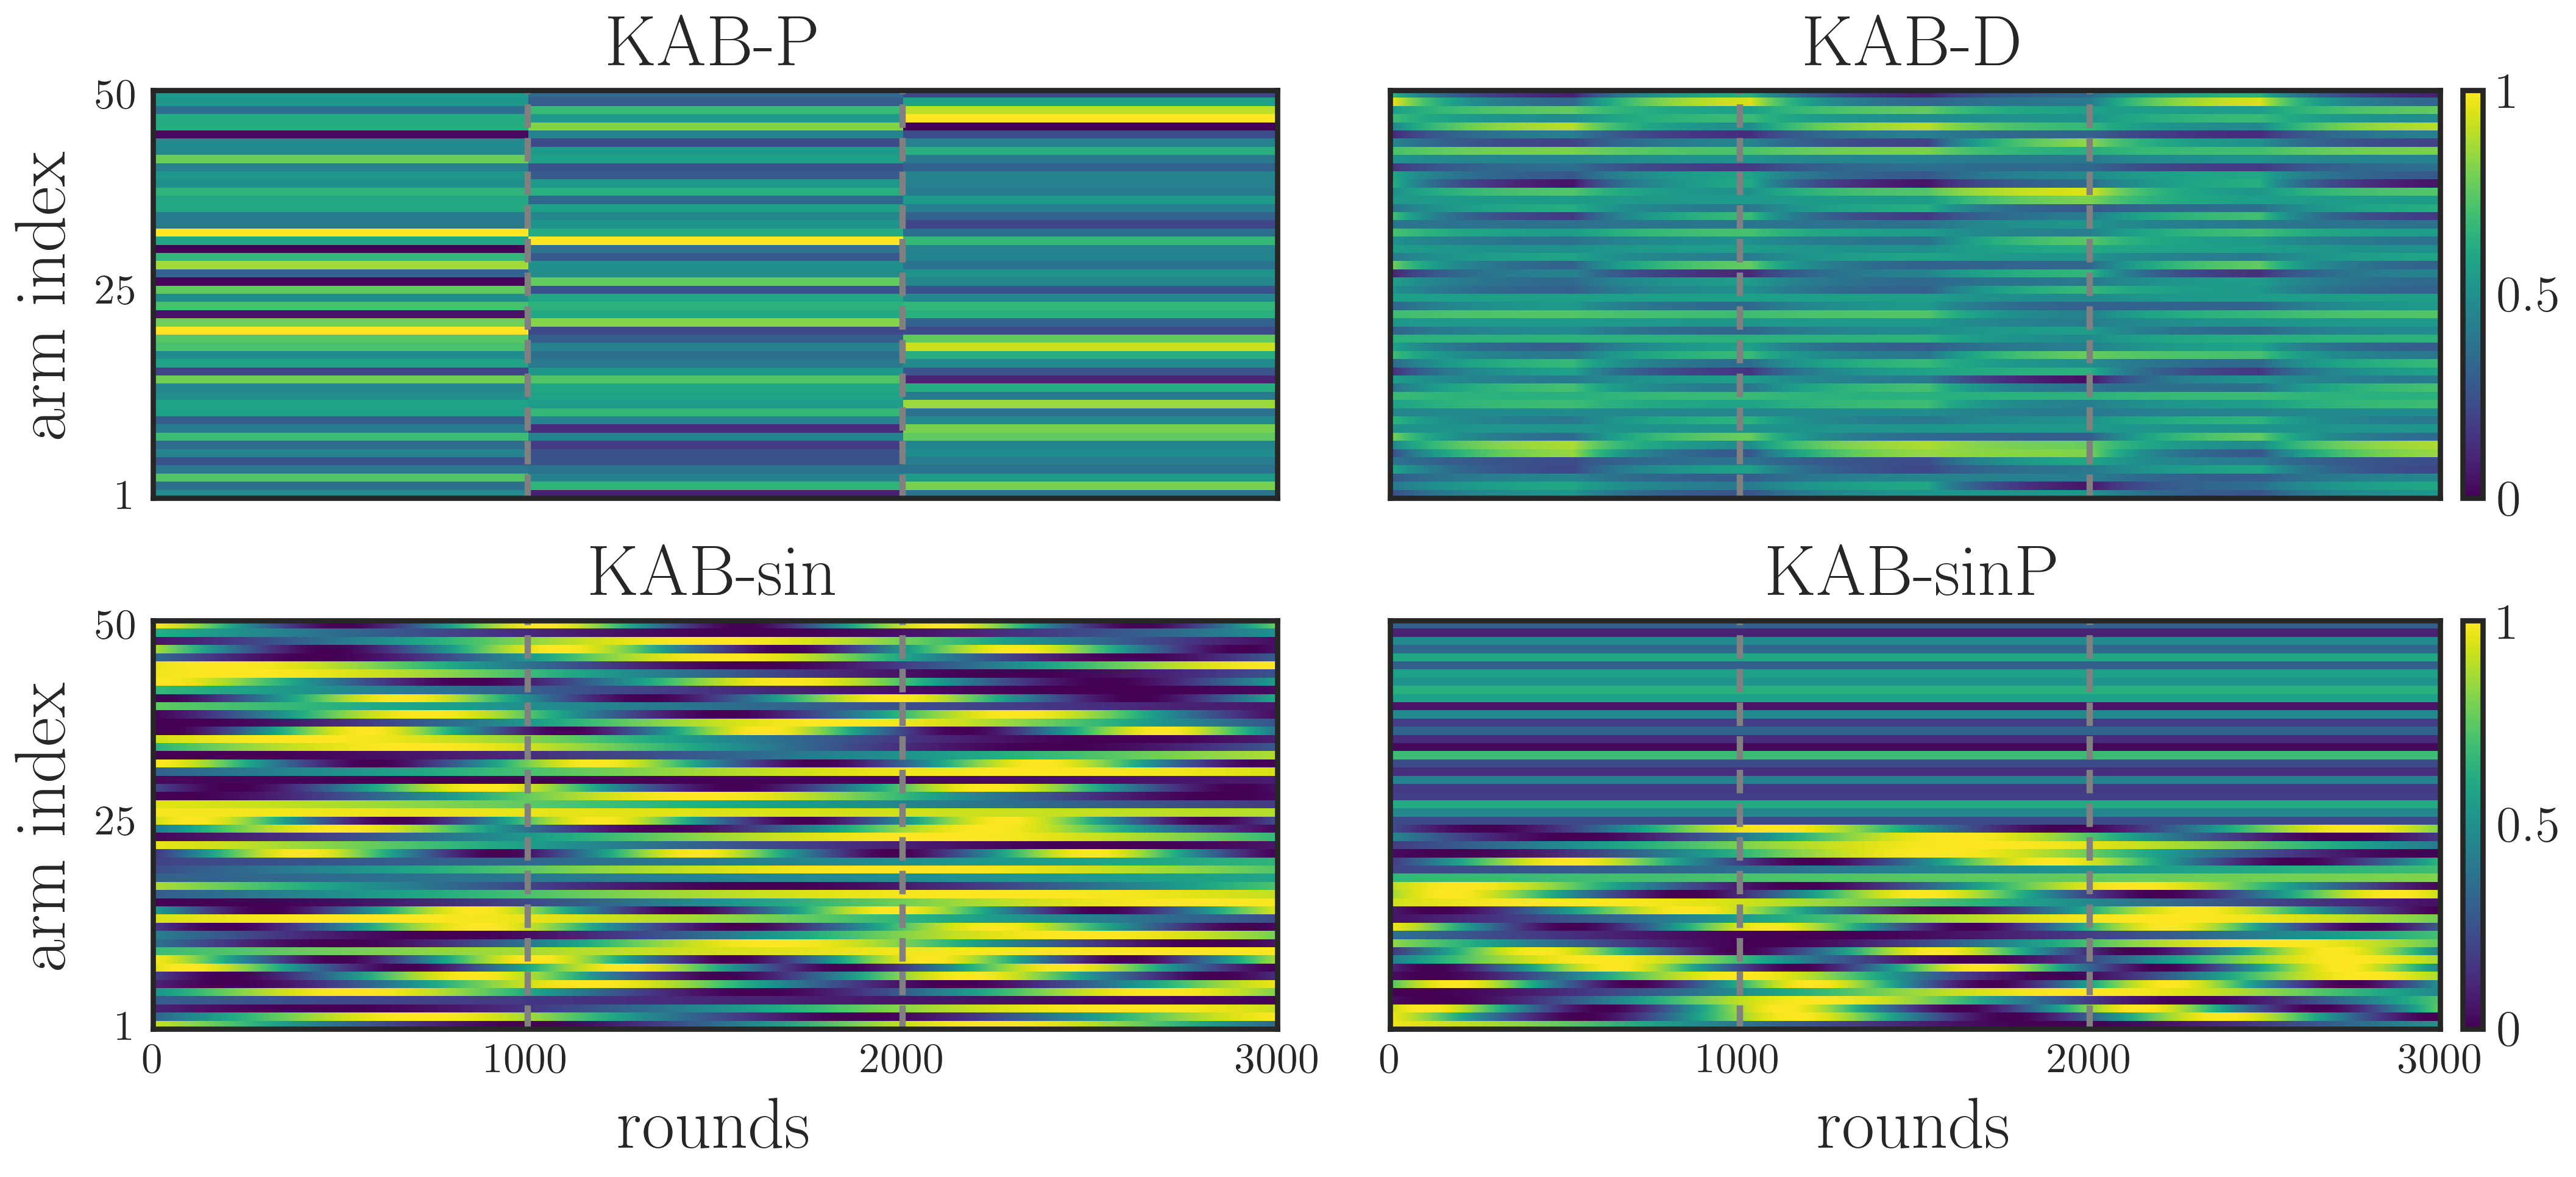
\includegraphics[width=1.\textwidth]{figures/envs_1.png}
    \caption{\textsc{Reward distribution for the four game variants} - \textit{The reward distribution for each arm and environment is plotted over two trials of 2000, demarcated by a dotted grey line.}}
    \label{fig:envs}
\end{figure}

% Results: scores and brief discussion
\subsection{Environment variants and number of arms}

The model has been tested and compared with the other algorithms: Thompson Sampling, Epsilon-Greedy, and UCB, in the four different variants of the K-armed bandit problem.
In figure \ref{fig:perf_plot}, it is reported their results over a different number of arms, ranging from 5 to 1000.
Overall, our model displayed a good performance over all environments and arm numbers, suffering only when the latter reached 1000.

\begin{figure}[H]
    \centering
    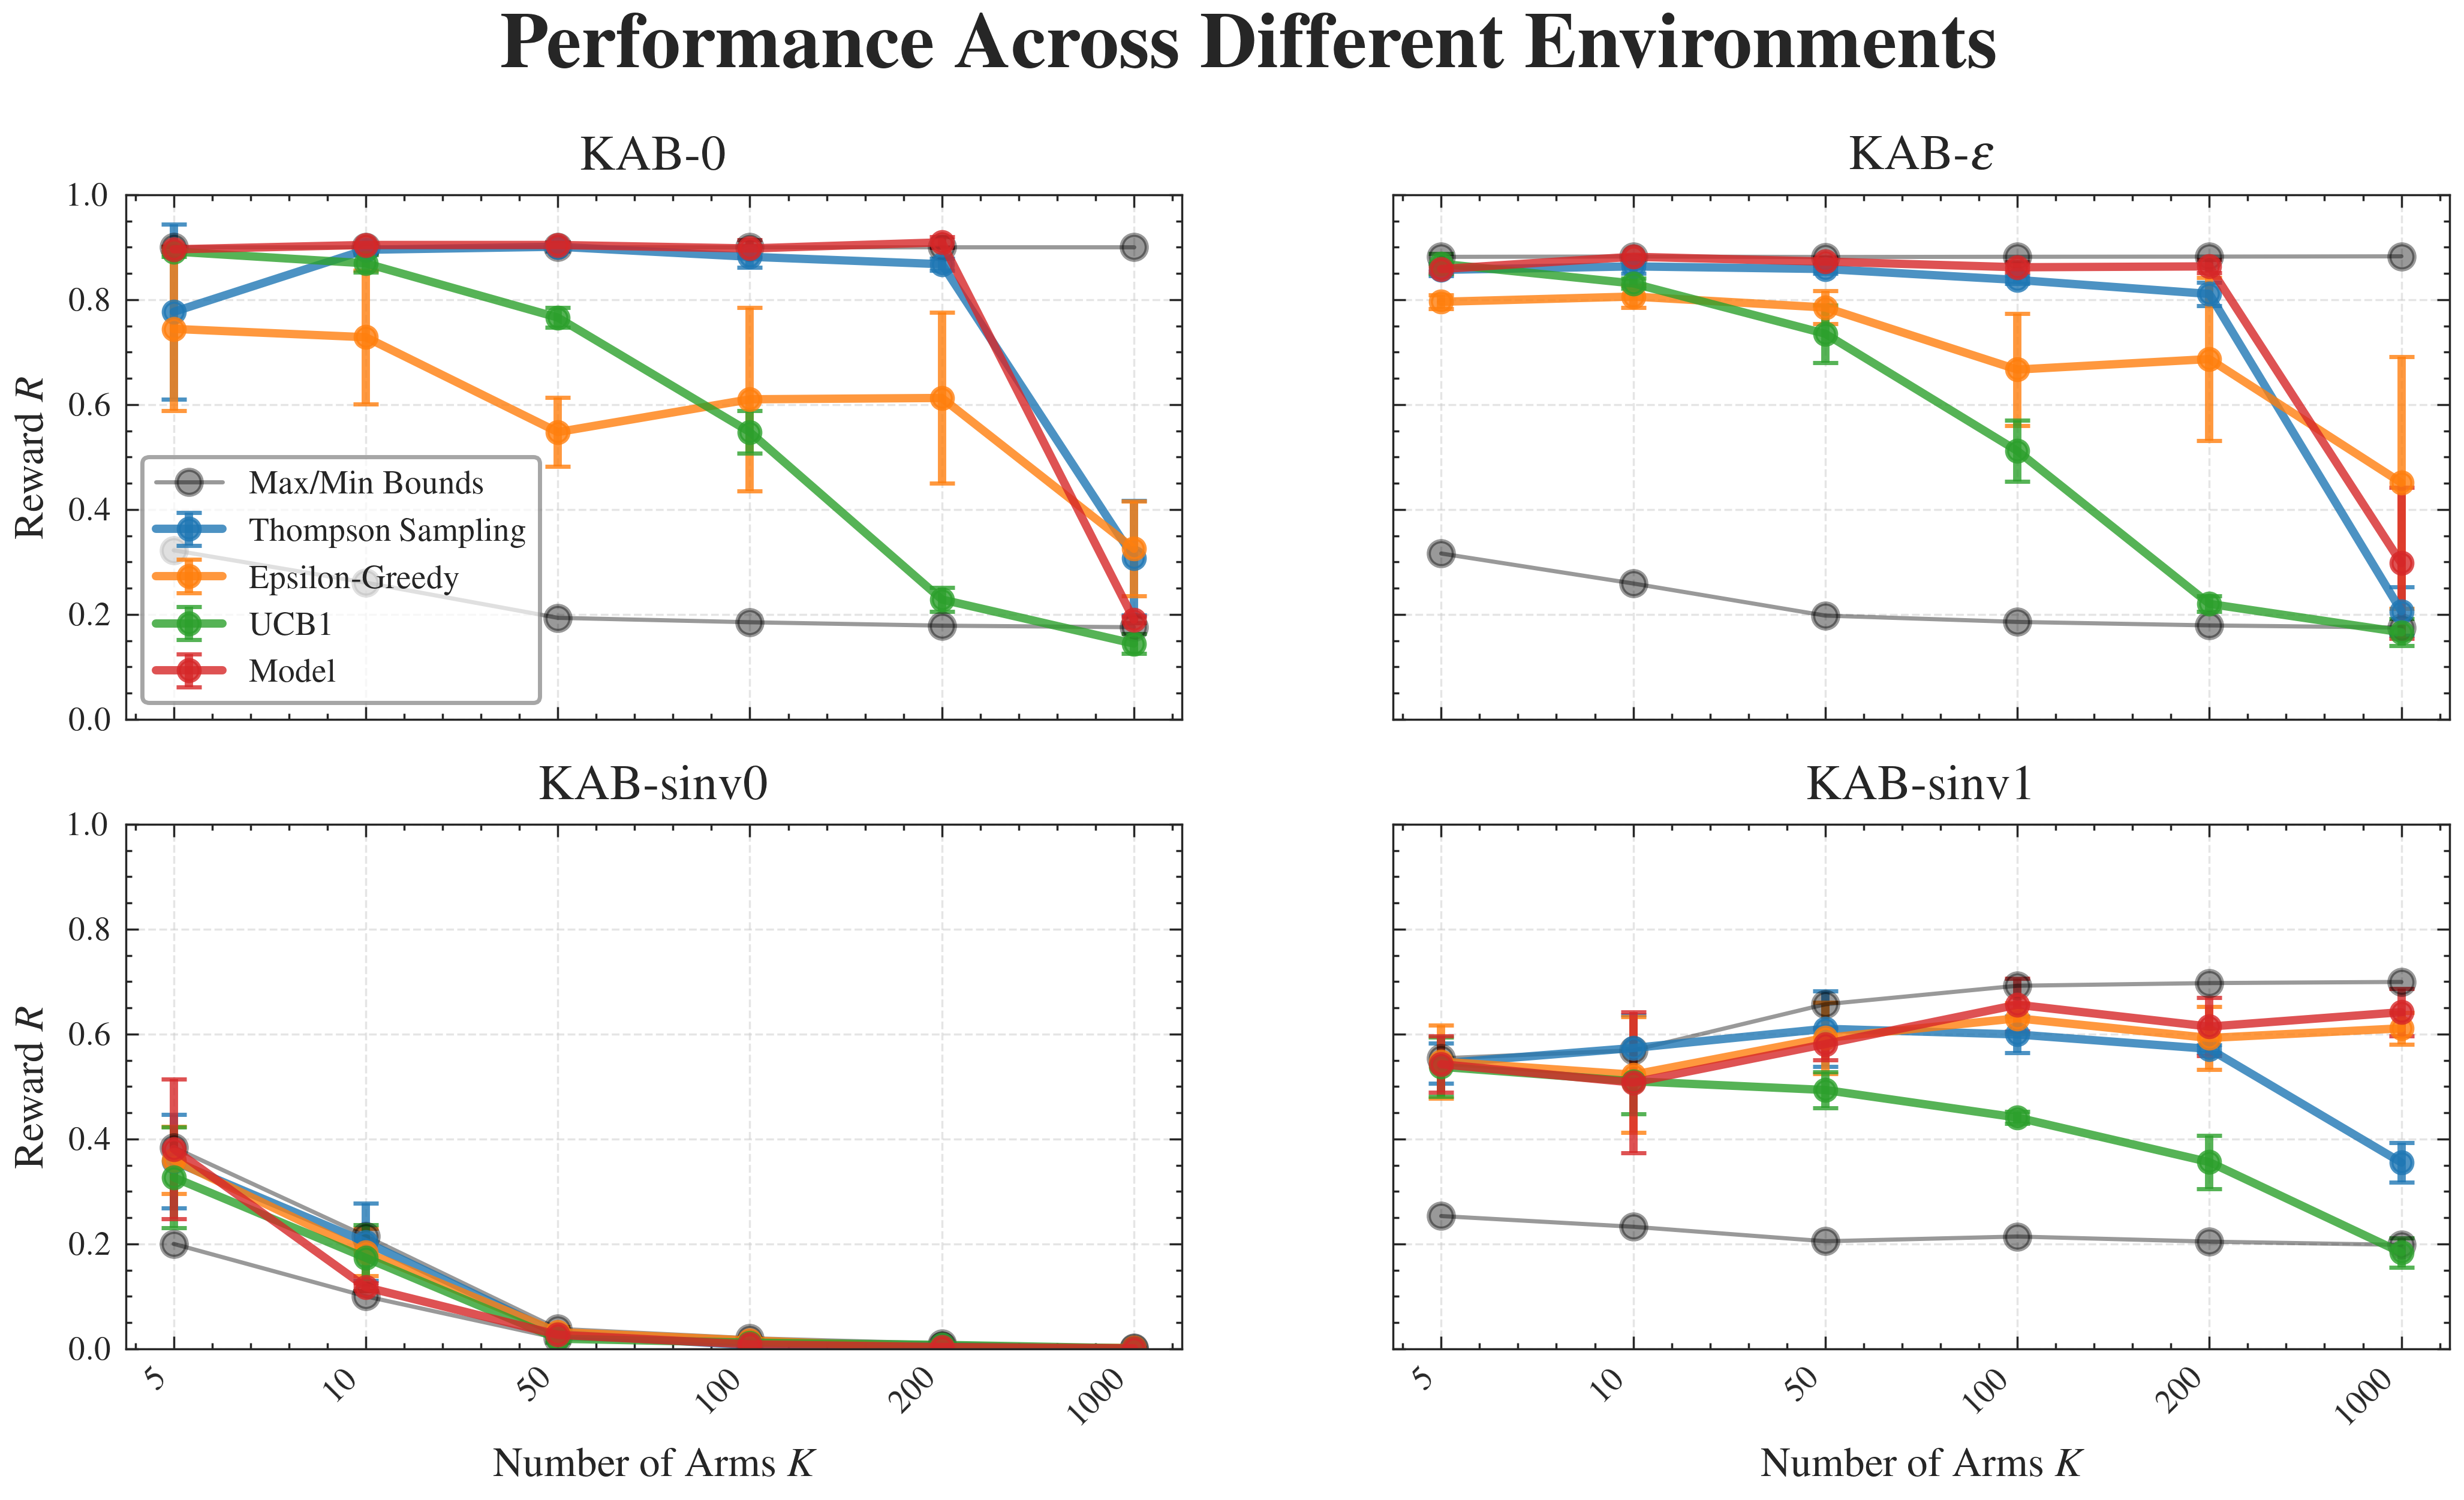
\includegraphics[width=1.\textwidth]{figures/performance_plot.png}
    \caption{\textsc{Performance comparison for different values of $K$ and game variants} - \textit{The models are evaluated on the four variants of the bandit problem, and their performance is measured as the average reward obtained over 2 trials of 2000 rounds each.}}
    \label{fig:perf_plot}
\end{figure}


% How the models work and compare
\subsection{Decision-making dynamics}

% entropy over rounds
\subsubsection{Entropy analysis}\label{sec:entropy}
\noindent For a better understanding of the qualitative differences between the models, we analyzed the progress over the rounds by tracking the selected arms in a simple piecewise stationary distribution environment.
The simulation was ran for $3$ trials with $2000$, and averaged over $5$ iterations.
Additionally, in order to quantify the variability of the decision policy at a given time and highlight the particularity of each decision-making behaviour, we calculated the entropy of the probability distribution $p$ of chosen arms, calculated over a window of 20 rounds, as $H=-\sum^{K}_{i} p_{i}\log(p_{i})$.
The unit of entropy is in nats, and it ranges from $0$ (no uncertainty) to $\log_{e}(K)$ (maximum uncertainty).
In figure \ref{fig:entropy_fig1}, it is plotted for each model the raster plot of selected arms together with its level of entropy. The reward probability distribution over the arms has an average of $H=2.02$.

As expected, the shape of the entropy curve expresses the inherent strategy adopted by each model.
In particular, the UCB algorithm showed the highest variability, marked by a persistent exploratory behaviour throughout the trials despite converging to reward options. Thompson Sampling was able to reach most solutions, although with difficulty in adapting to new reward distributions
leading to high entropy levels.
$\epsilon-$Greedy also showed a good performance quite reliably, with the greedy strategy assuring low entropy for most of the rounds.
Similar behaviour was observed for our model, which was able to reach the optimal policy and maintain it over time, with entropy peaking mostly at the beggining of the trials and being, on average, the lowest among all models.
Indeed, the dynamics of our model make it particularly suited for the task of non-stationary K-armed bandits, as it is able to quickly adapt to new reward distributions and firmly maintain a greedy policy.

\begin{figure}[H]
    \centering
    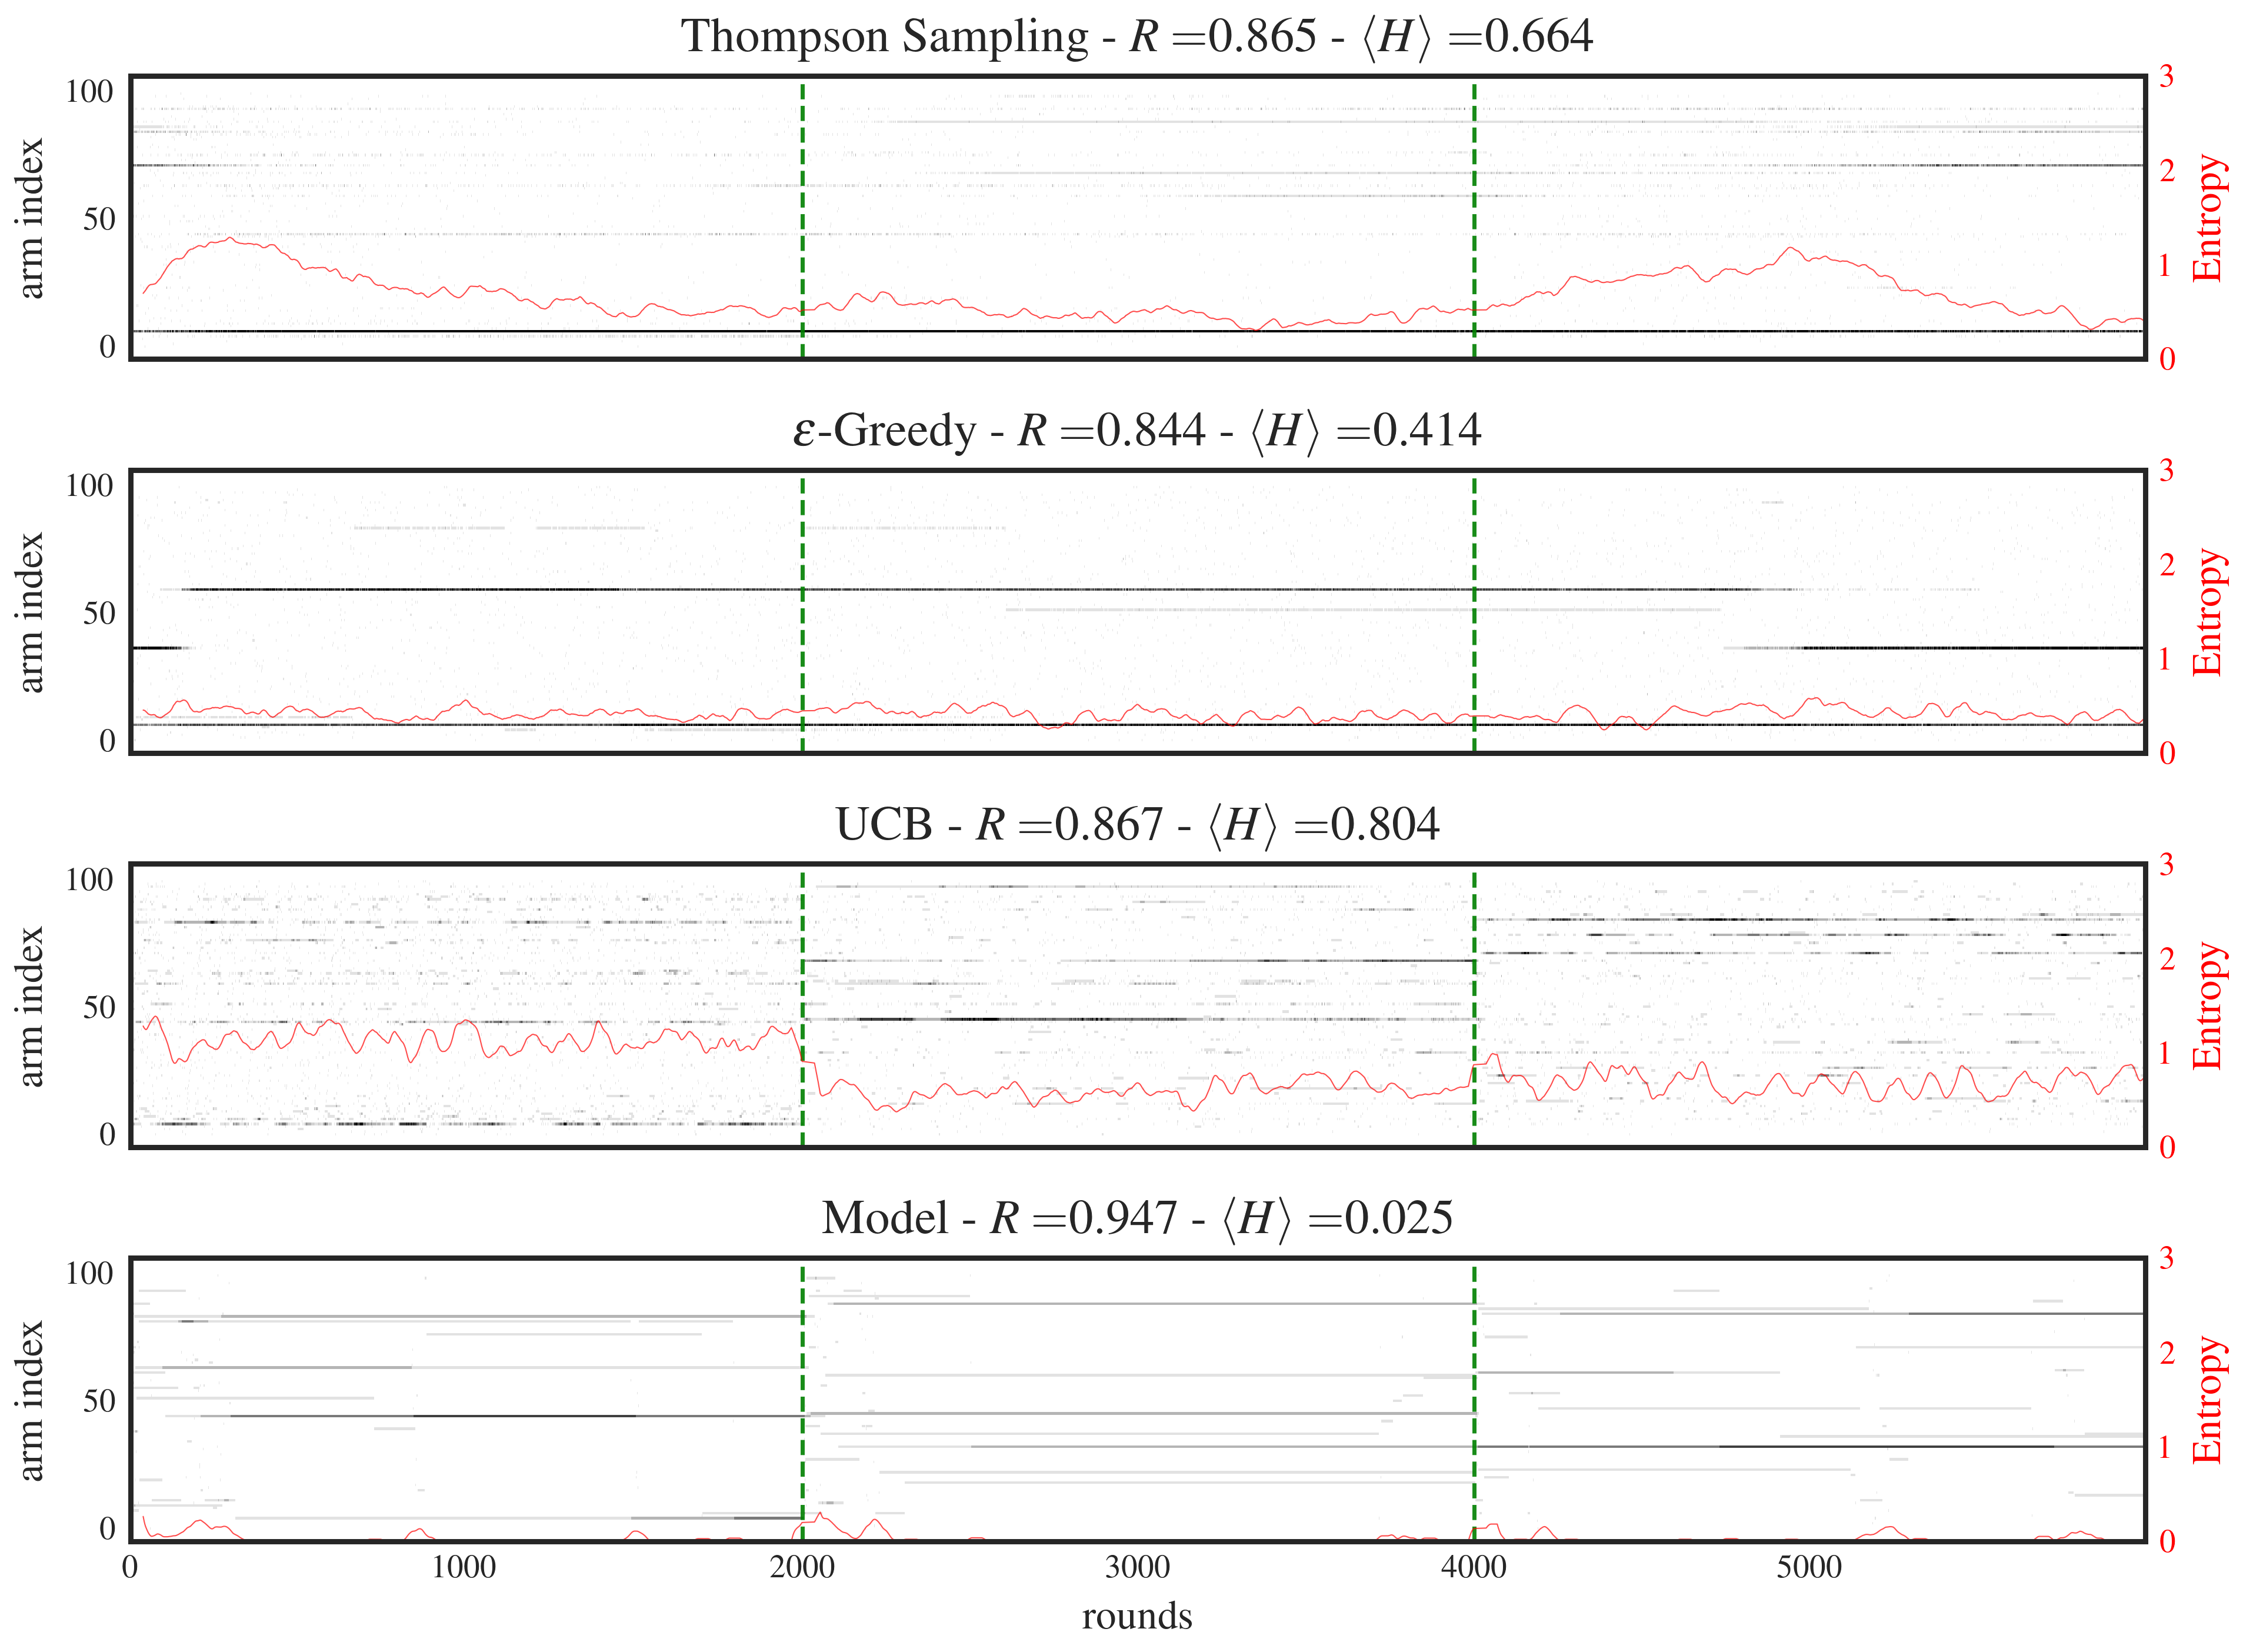
\includegraphics[width=1.0\textwidth]{figures/performance_analysis_v0_1.png}
    \caption{\textsc{Decision-making dynamics for different models} \textit{Each plot display the results from one model. The raster plots (black dots) show the arms selected at each round.
The red lines represent the entropy level, calculated from the distribution of selections over the preceeding 20 rounds, smoothed with a 30-steps moving average. In the plot titles, the total reward and average entropy over all trials are also reported.}}
    \label{fig:entropy_fig1}
\end{figure}


% how robust and structure is the model
\subsubsection{Robustness}

% robustness
\noindent Then, we sought to investigate the robustness of the model, quantified as the capacity to endure increasing levels of entropy in the reward distribution.
The simulation was done in a piecewise stationary environment with $K=50$, averaged over 128 independent runs.
The results report how all models are capable of robust performance even in the presence of high uncertainty.
In the top row of figure \ref{fig:entropy_distr}, it is plotted the average reward obtained by each model against the reward distribution entropy in two trials.
In the second trial however, there is a ubiquitous and clear decline in rounds with elevated entropy. This can be explained by the greater challenge of switching arms when numerous options appear similarly good.
In general, our model shows to perform as good as UCB, and better than $\epsilon$-Greedy and Thompson Sampling.
Further, the latter seemed to suffer the most, probably due to its conservative approach and difficulty of disengaging from an previously rewarding arm, as underlined also in figure \ref{fig:entropy_fig1}.
In the same figure, the regret (dashed lines) tells the same story, and remarks the robust performance over uncertainty.

Another perspective to this analysis is given by the plots in the bottom row, which show the average entropy of the selections.
Overall, there is the not suprising trend of increasing selection entropy with the entropy of the reward distribution. However, striking is the exception of Epsilon-Greedy, which maintain a constant level throughout.
On the one hand, UCB shows a marked and gradual increase, while Thompson Sampling follows with some delay.
On the other hand, our model display a more abrupt change, \textbf{at around 2.43 nats}, going from a state of very low to very high entropy.
For more details about the distribution see the appendix \ref{sec:appendix_entropy}.


\begin{figure}[H]
    \centering
    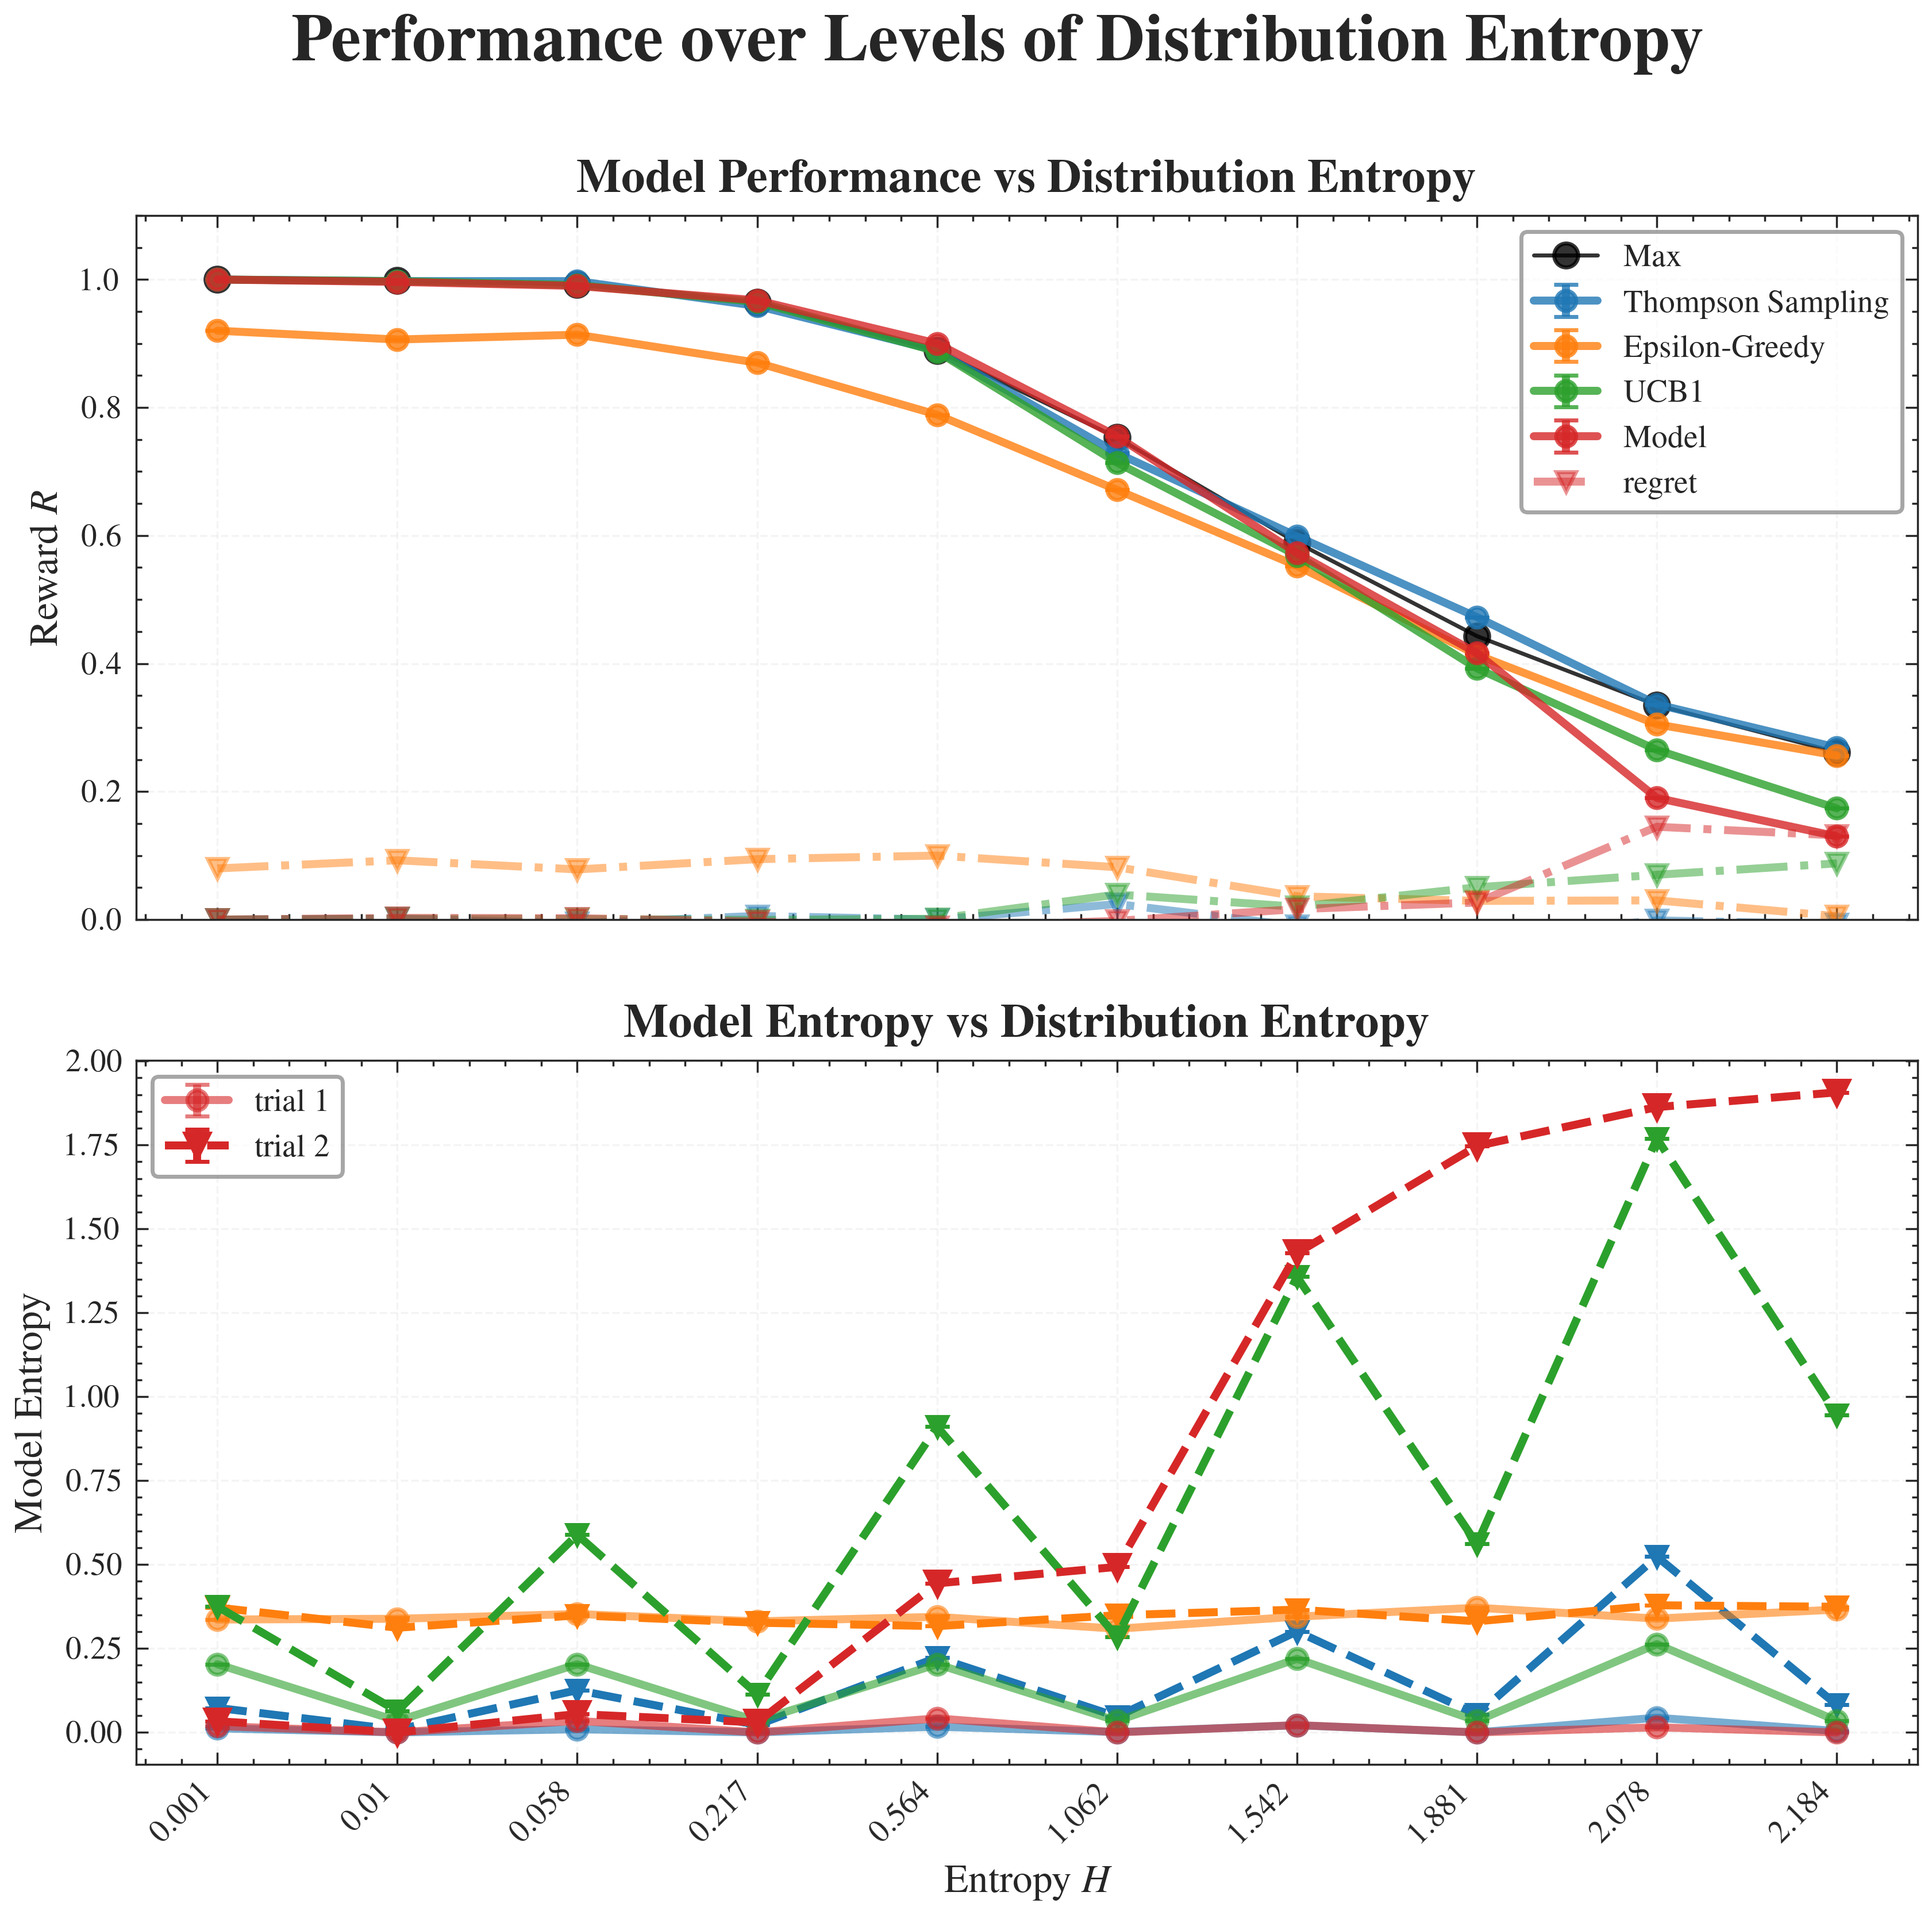
\includegraphics[width=0.9\textwidth]{figures/entropy_performance_plot.png}
    \caption{\textsc{Entropy analysis for the model in a stationary setting} - Top row: \textit{trial 1 and 2 have been divided into two columns. A solid line represents the average reward obtained by a model for increasing levels of entropy (in nats) in the reward distribution; a dashed line instead reports the regret with respect to the upper bound (black solid line) }
- Bottom row: \textit{average entropy of the selections for the first and second trial of the simulation, each with 2000 rounds each (as calculated in \ref{sec:entropy}).}}
\end{figure}\label{fig:entropy_distr}






\newpage


\section{Discussion}


% work on the k-armed bandit problem and neuroscience
In the context of human behaviour, it has been observed that the adopted policies vary considerably \cite{steyversBayesianAnalysisHuman2009a}. However, the subjects seems able to integrate environmental uncertainty and trial generalization in their strategy, and Bayesian algorithms are generally a good fit for the observed behaviour \cite{schulzFindingStructureMultiarmed2020, zhangForgetfulBayesMyopic2013}.






\newpage

% Acknowledgements & Statements
This work was supported by the European Union (\#add more).
\hfill \break
The authors declare no competing interests.
\hfill \break
The code is publicly available and can be found at
\url{https://github.com/iKiru-hub/minBandit.git} (\#change to Zenodo).

%print bibliography
\bibliography{navmem_refs}

\newpage


\section{Appendix}\label{sec:appendix}


\subsection{Gaussian-sigmoid function}
\noindent The function $\Phi_{\cdot}$ is defined by combining a generalized version of the sigmoid, namely with a gain $\beta \neq 1$ and offset $\alpha\neq 0$, and a Gaussian with mean $\mu$ and variance $\sigma^{2}$. Their contributions are weighted by as $r$ and $1-r$ ($r\in(0,1)$) respectively.

\begin{equation*}
    \Phi_v(x) = r\left(1 + \exp^{-\beta(x-\alpha)}\right)^{-1} + (1-r)\exp\left(-\frac{(x-\mu)^2}{2\sigma^2}\right)
\end{equation*}

\noindent The motivation behind this choice is to express a function that possesses a bounded region (depending on $\mu,\,\sigma$) at a high/low peak (depeding on the value of $\gamma_{2}$), and a continuous transition to a constant value (depending on the steepness of the sigmoid $\beta$, shift
$\alpha$, and intensity $\gamma_{1}$).

\begin{figure}[ht]
    \centering
    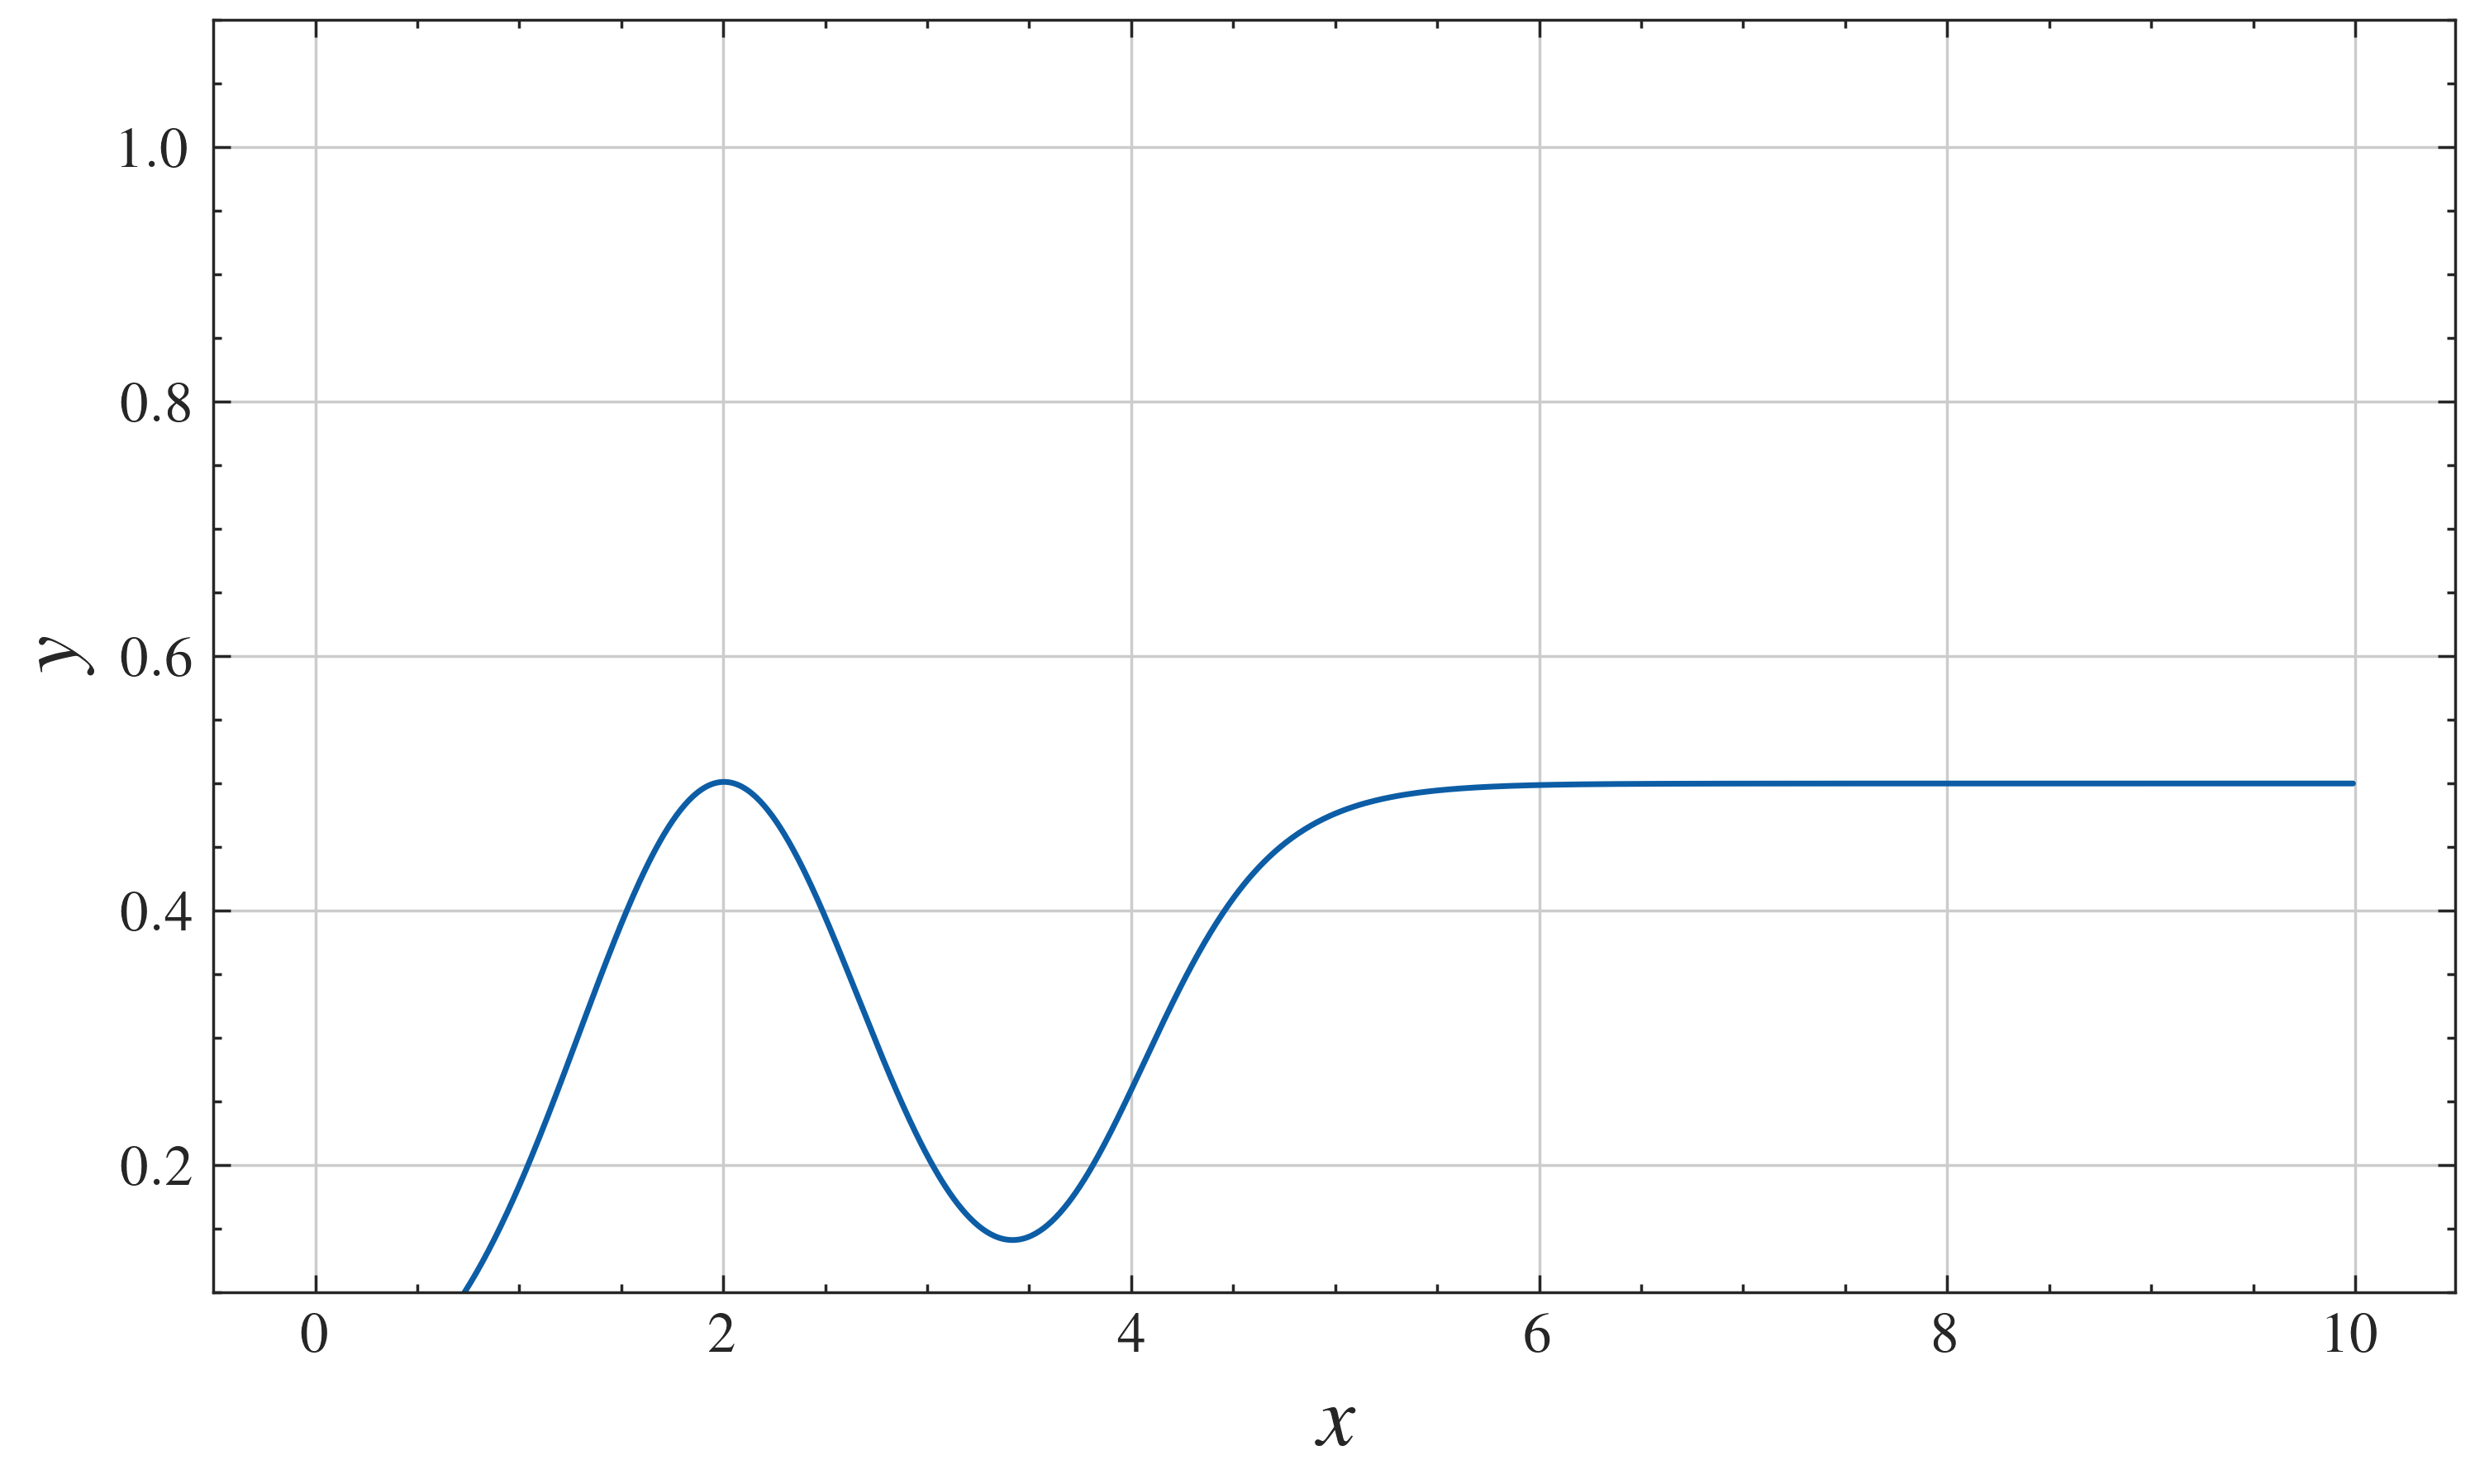
\includegraphics[width=0.8\textwidth]{figures/gaussian_sigmoid.png}
    \caption{\textsc{Activation function $\Phi_{v}$} - \textit{Parameters $\beta=10$, $\alpha=1$, $\mu=1$, $\sigma=1$, and $r=0.5$.}}
    \label{fig:gau_sigm}
\end{figure}


\subsection{Evolution search}
The optimization was carried out over several parameters concerning the model architecture and dynamics:
\textbf{Network parameters}
\begin{itemize}
    \item $\tau_{u}$: time constant of population $u$ ($M$)
    \item $\tau_{v}$: time constant of population $v$ ($V$)
    \item $g$: gain of the sigmoidal activation function of population v
    \item $\theta$: threshold of the sigmoidal activation function of population v
    \item $W^{+}$: maximal weight value for the weights $\textbf{W}^{MV}$
\end{itemize}

\noindent \textbf{Option value function parameters}
\begin{itemize}
    \item $\beta_{v}$: steepness of the sigmoid
    \item $\alpha_{v}$: shift of the sigmoid
    \item $\mu_{v}$: mean of the Gaussian
    \item $\sigma_{v}$: variance of the Gaussian
    \item $r_{v}$: weight of the sigmoid
\end{itemize}

\noindent \textbf{Learning rate function parameters}
\begin{itemize}
    \item $\gamma_{\eta}$: intensity of the l
    \item $\beta_{\eta}$: steepness of the sigmoid
    \item $\alpha_{\eta}$: shift of the sigmoid
    \item $\mu_{\eta}$: mean of the Gaussian
    \item $\sigma_{\eta}$: variance of the Gaussian
    \item $r_{\eta}$: weight of the sigmoid
\end{itemize}

\noindent Each individual has been evaluated over environment the following environments:

\begin{itemize}
    \item \textsc{MAB-0}: average reward distribution entropy $\langle H\rangle=2.05$
    \item \textsc{KAB-$\sin$P}: average reward distribution entropy $\langle H\rangle=2.1$, given $K$ arm frequencies $f_{k}$ as an equally spaced set $\{0.1\ldots i\ldots 0.4\}$, phases $\lambda_{k}$ drawn from an uniform $\sim \mathcal{U}(0, 2\pi)$, and half of the arms have been set to constant values drawn from
        another uniform $\sim \mathcal{U}(0.1, 0.7)$; the final reward distribution was not normalized.
\end{itemize}

\noindent The number of arms was $K=10$ and $150$, and lasted for $2$ trials with $2000$ rounds each.
The final fitenss was the average over $2$ iterations.

\hfill \break
The optimization has been implemented in Python using the \texttt{DEAP} library, and the algorithm used was the \texttt{CMA-ES} algorithm. The optimization involved $70$ generations with a population size of $128$ individuals. The mutation rate was set to $0.5$ with a sigma of $0.8$, the cross-over rate was set to $0.4$.
The run were carried out on a 256-core AMD EPYC 7763 with 2TB of RAM.


\subsection{Reward distribution entropy}\label{sec:appendix_entropy}

\noindent The calculation of a set of $N$ reward probability distribution $\mathbf{p}_{i}\text{  for  } i\ldots N$ for $K$ values with a progressively decreasing levels of entropy $\mathbf{h}_{i}\text{  for  } i\ldots N$ has been obtained by the following algorithm:

\begin{algorithm}[ht]
\caption{Reward Probability Distribution Generation}
\label{alg:reward_distribution}
\SetAlgoLined
\KwIn{Number of distributions $N$, dimension $K$}
\KwOut{Set of probability distributions ${\mathbf{p}_i}$ with decreasing entropy}
\SetKwComment{Comment}{// }{ }
\textbf{Initial Setup:}
Define set $B = \{1.5^x \mid x = 1, \ldots, 7\}$; \\
\For{$i \gets 1$ to $N$}{
$\mathbf{z} \gets \text{RandomVector}(0,1)^K$;\\
$j \gets \text{RandomIndex}(K)$;\\
$\mathbf{z}_j \gets 1$;\\
$\beta_i \gets \text{Sample index=} i \text{ from }(B)$ \Comment*[r]{Sample temperature from $B$}

$\mathbf{p}_i \gets \frac{\exp(\beta_i \mathbf{z})}{\sum_j \exp(\beta_i \mathbf{z}_j)}$ \Comment*[r]{Softmax with temperature}
}
\Return ${\mathbf{p}_i}$
\end{algorithm}


\subsection{Table of results}

% --- table K.5
\begin{table}[H]
\centering
\caption{Performance comparison for $K=5$}
\label{tab:k5}
\begin{tabular}{l c c c}
\toprule
\textbf{Model} & \textbf{\textsc{KAB-0}} & \textbf{\textsc{KAB-$\epsilon$}} & \textbf{\textsc{KAB-$\sin$}}\\
\midrule
Optimal & $0.900$ & $0.881$ & $0.563$ \\
Random & $0.330$ & $0.337$ & $0.200$ \\
\midrule
Thompson & $0.905$ & $0.617$ & $0.317$ \\
$\epsilon$-Greedy & $0.797$ & $0.531$ & $0.315$ \\
UCB & $0.897$ & $0.656$ & $0.319$ \\
\textbf{Model} & $\mathbf{0.899}$ & $\mathbf{0.663}$ & $\mathbf{0.265}$ \\

\bottomrule
\end{tabular}
\end{table}

% --- table K.10
\begin{table}[H]
\centering
\caption{Performance comparison for $K=10$}
\label{tab:k10}
\begin{tabular}{l c c c}
\toprule
\textbf{Model} & \textbf{\textsc{KAB-0}} & \textbf{\textsc{KAB-$\epsilon$}} & \textbf{\textsc{KAB-$\sin$}} \\
\midrule
Optimal & $0.900$ & $0.885$ & $0.355$  \\
Random & $0.247$ & $0.250$ & $0.100$ \\
\midrule
Thompson & $0.896$ & $0.648$ & $0.339$ \\

$\epsilon$-Greedy & $0.611$ & $0.597$ & $0.343$ \\
UCB & $0.891$ & $0.655$ & $0.358$ \\
\textbf{Model} & $\mathbf{0.905}$ & $\mathbf{0.668}$ & $\mathbf{0.203}$  \\
\bottomrule
\end{tabular}
\end{table}

% --- table K.100
\begin{table}[H]
\centering
\caption{Performance comparison for $K=100$}
\label{tab:k100}
\begin{tabular}{l c c c}
\toprule
\textbf{Model} & \textbf{\textsc{KAB-0}} & \textbf{\textsc{KAB-$\epsilon$}} & \textbf{\textsc{KAB-$\sin$}} \\
\midrule
Optimal & $0.900$ & $0.883$ & $0.020$  \\
Random & $0.196$ & $0.201$ & $0.010$ \\
\midrule
Thompson & $0.894$ & $0.586$ & $0.013$ \\
$\epsilon$-Greedy & $0.519$ & $0.574$ & $0.018$ \\
UCB & $0.853$ & $0.572$ & $0.012$ \\
\textbf{Model} & $\mathbf{0.898}$ & $\mathbf{0.651}$ & $\mathbf{0.010}$  \\
\bottomrule
\end{tabular}
\end{table}

% --- table K.200
\begin{table}[H]
\centering
\caption{Performance comparison for $K=100$}
\label{tab:k200}
\begin{tabular}{l c c c}
\toprule
\textbf{Model} & \textbf{\textsc{KAB-0}} & \textbf{\textsc{KAB-$\epsilon$}} & \textbf{\textsc{KAB-$\sin$}} \\
\midrule
Optimal & $0.900$ & $0.885$ & $0.010$  \\
Random & $0.178$ & $0.176$ & $0.005$ \\
\midrule
Thompson & $0.875$ & $0.624$ & $0.006$ \\
$\epsilon$-Greedy & $0.679$ & $0.588$ & $0.010$ \\
UCB & $0.792$ & $0.510$ & $0.006$ \\
\textbf{Model} & $\mathbf{0.905}$ & $\mathbf{0.610}$ & $\mathbf{0.006}$  \\
\bottomrule
\end{tabular}
\end{table}

% --- table K.1000
\begin{table}[H]
\centering
\caption{Performance comparison for $K=100$}
\label{tab:k1000}
\begin{tabular}{l c c c}
\toprule
\textbf{Model} & \textbf{\textsc{KAB-0}} & \textbf{\textsc{KAB-$\epsilon$}} & \textbf{\textsc{KAB-$\sin$}} \\
\midrule
Optimal & $0.900$ & $0.880$ & $0.002$  \\
Random & $0.177$ & $0.178$ & $0.001$ \\
\midrule
Thompson & $0.779$ & $0.445$ & $0.001$ \\
$\epsilon$-Greedy & $0.386$ & $0.478$ & $0.002$ \\
UCB & $0.301$ & $0.185$ & $0.001$ \\
\textbf{Model} & $\mathbf{0.703}$ & $\mathbf{0.480}$ & $\mathbf{0.001}$  \\
\bottomrule
\end{tabular}
\end{table}


\newpage


\end{document}





